\documentclass{beamer}
 
\usepackage[utf8]{inputenc}
\usepackage{tabularx}
\usepackage{graphicx}
 
\usetheme{Copenhagen}
 
\defbeamertemplate*{footline}{shadow theme}{%
	\leavevmode%
	\hbox{\begin{beamercolorbox}[wd=.5\paperwidth,ht=2.5ex,dp=1.125ex,leftskip=.3cm plus1fil,rightskip=.3cm]{author in head/foot}%
			\usebeamerfont{author in head/foot}\hfill\insertshortauthor
		\end{beamercolorbox}%
		\begin{beamercolorbox}[wd=.4\paperwidth,ht=2.5ex,dp=1.125ex,leftskip=.3cm,rightskip=.3cm plus1fil]{title in head/foot}%
			\usebeamerfont{title in head/foot}\insertshorttitle\hfill%
		\end{beamercolorbox}%
		\begin{beamercolorbox}[wd=.1\paperwidth,ht=2.5ex,dp=1.125ex,leftskip=.3cm,rightskip=.3cm plus1fil]{title in head/foot}%
			\usebeamercolor{title in head/foot} \hfill\insertframenumber\,/\,\inserttotalframenumber
		\end{beamercolorbox}}%
		\vskip0pt%
}
 
%Information to be included in the title page:
\title[Architectural Change in CI Builds]{Impact of Architectural Change on Continuous Integration Build Outcome}
\author{Johannes K{\"a}stle}
\institute{University of Alberta}
\date{12/07/2017}
 
\begin{document}

\begin{frame}
	\titlepage
	
	\begin{center}
		\url{https://github.com/jodokae/cmput663-architecture}
	\end{center}
\end{frame}

\section{Introduction}
\subsection{Motivation}
\begin{frame}
\frametitle{Motivation}

\begin{itemize}
	\item Explore Architectural Change in Open-Source Projects
	\item Decrease Number of Failing Builds
	\item Increase Productivity
\end{itemize}

\pause

\begin{block}{Research Question}
Does change in architecture influence the outcome of a CI build?
\end{block}

\end{frame}


\subsection{Background}
\begin{frame}
\frametitle{Background}

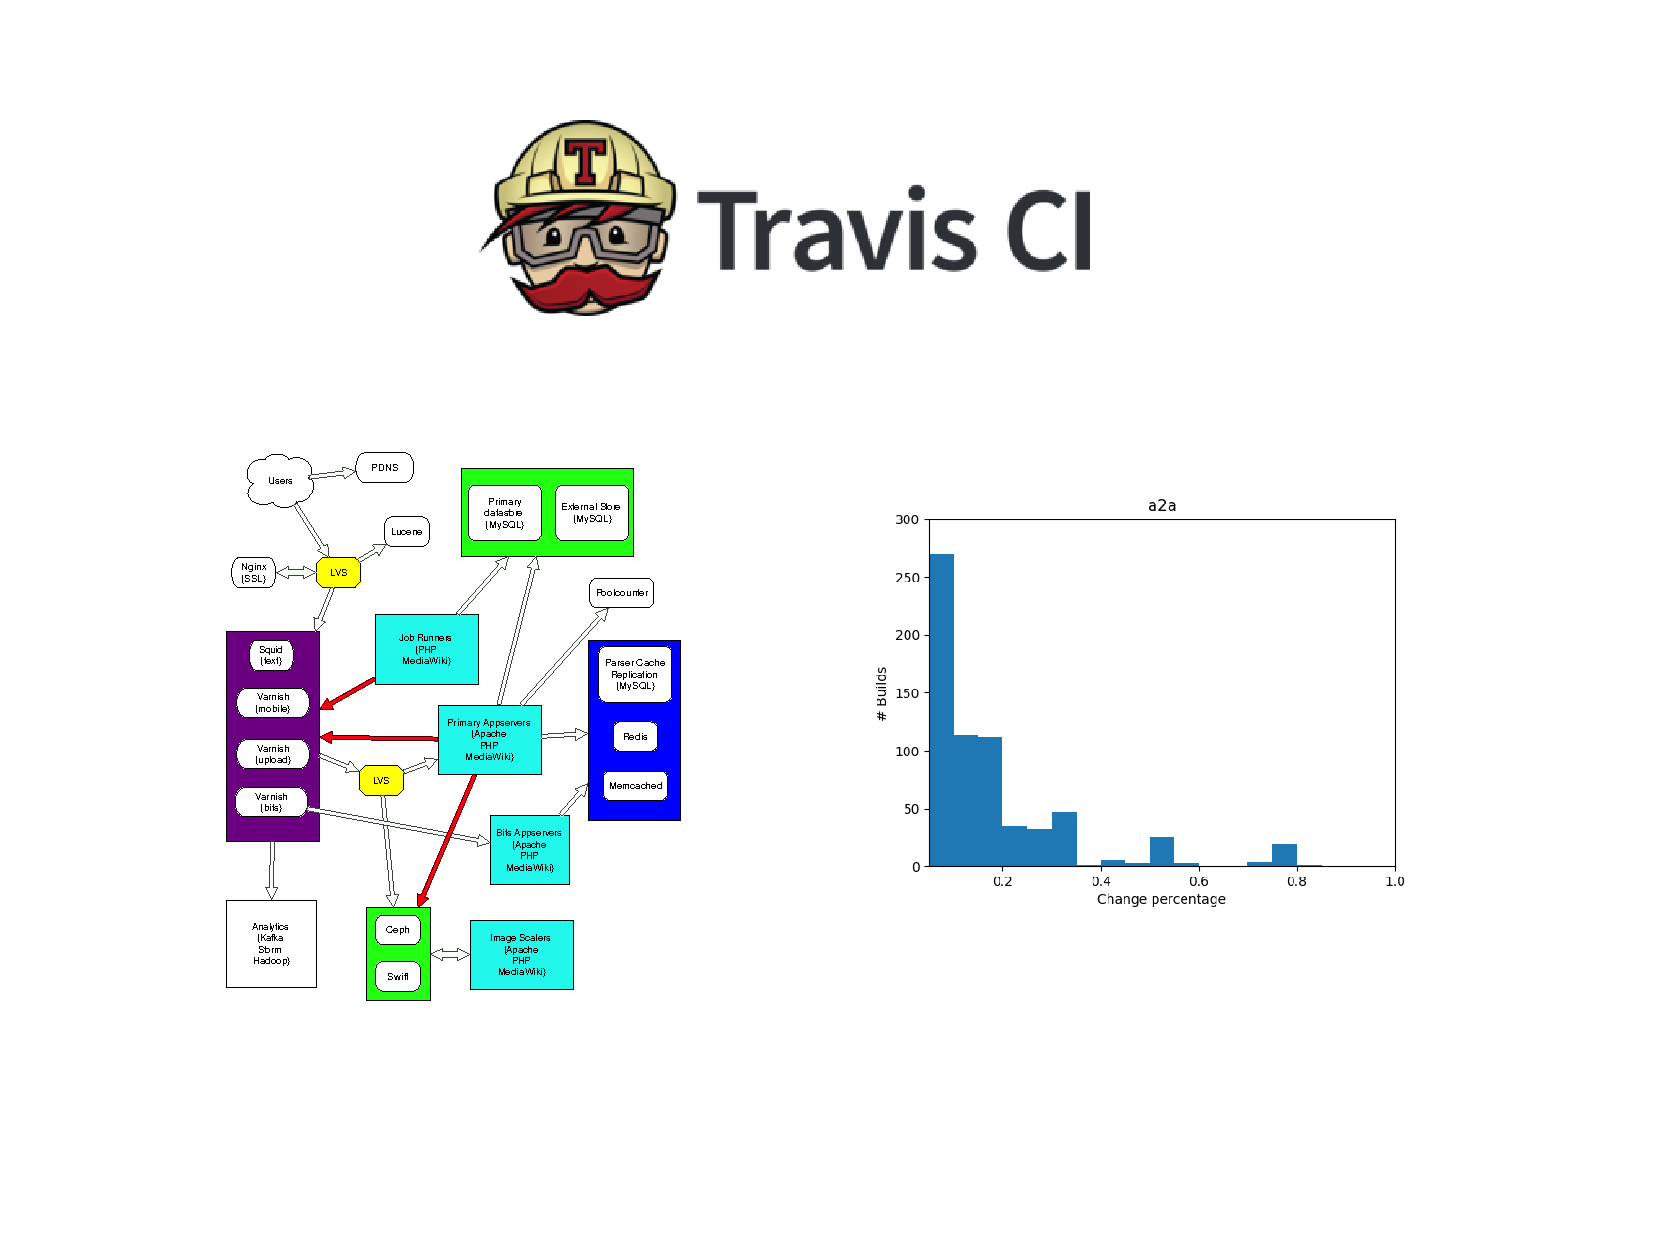
\includegraphics[width=11cm]{assets/Background.pdf}

\end{frame}

\subsection{Related Works}
\begin{frame}
\frametitle{Related Works}


\begin{itemize}
	\item Build Prediction
	\begin{itemize}
		\item Correlation in TravisTorrent
		\item Project / Person specific
		\item (Cascading) Tree Classifier
	\end{itemize}
	\pause
	\item Architecture
	\begin{itemize}
		\item Consistency
		\item Reconstruction
		\begin{itemize}
			\item HUSACCT
			\item ARCADE
		\end{itemize}
		\item Change
		\begin{itemize}
			\item Kernels
			\item ARCADE
		\end{itemize}
	\end{itemize}
\end{itemize}

\end{frame}

\begin{frame}
	\frametitle{HUSACCT}
	\framesubtitle{HU Software Architecture Complicane Checking}
	
	Leo Pruijt, HU University of Applied Sciences Utrecht
	
	\begin{itemize}
			\item Conformance Framework
			\item Java, C\#
			\item Extracts from Source Files
			\item Different Dependencies
			\item Needs Module Definition
	\end{itemize}

\end{frame}

\begin{frame}
	\frametitle{ARCADE}
	\framesubtitle{Architecture Recovery, Change, And Decay Evaluator }
	
	University of Southern California
	
	\begin{itemize}
		\item Software Workbench
		\item Java, C, C++
		\item Reconstructors
		\begin{enumerate}
			\item ACDC - Pattern Based
			\item ARC - Semantic Based
		\end{enumerate}
		\item Change Metrics
		\begin{enumerate}
			\item a2a
			\item cvg
		\end{enumerate}
	\end{itemize}
		
\end{frame}

\begin{frame}
	\frametitle{ARCADE}
	\framesubtitle{Metrics}
	
		\[
		a2a(A_i, A_j) = 1 - \frac{mto(A_i, A_j)}{aco(A_i) + aco(A_j)}
		\]
		
		$mto(A_i, A_j)$ steps from $A_i$ to $A_j$
		
		$aco(A_i)$ = steps to create $A_i$
		
		\pause
		
		\[
		cvg(A_i, A_j) = \frac{|simC(A_i, A_j)|}{|allC(A_i)|}
		\]
		
		$simC(A_i, A_j)$ is number of clusters with $c2c >$ threshold. 
		
		\[
		c2c(c_i, c_j) = \frac{|\text{entities}(c_i) \cap \text{entities}(c_j)|}{\max(|\text{entities}(c_i)|, |\text{entities}(c_j)|)}
		\]
\end{frame}

\begin{frame}
	\frametitle{Martin's Metrics}
	
	\begin{itemize}
		\item Afferent Coupling A
		\item Efferent Coupling E
		\item Instability $I = \frac{E}{A + E} $
	\end{itemize}
	
\end{frame}

\section{Architectural Change on Build Outcome}
\subsection{Methodology}
\begin{frame}
\frametitle{Methodology}

\begin{block}{Toolchain}
	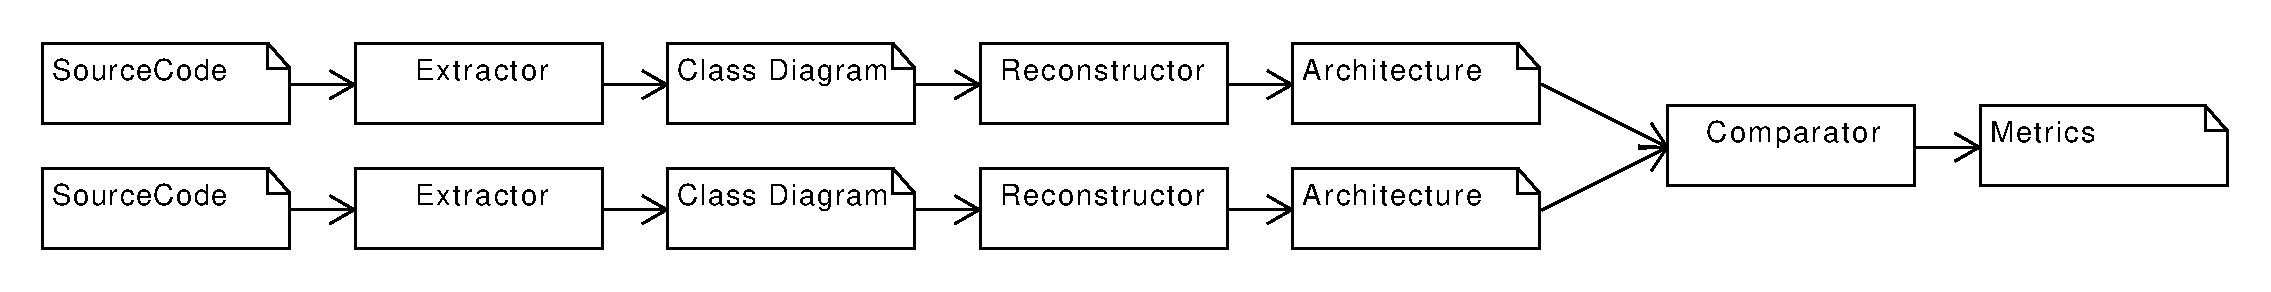
\includegraphics[width=10cm]{assets/overview.pdf}
\end{block}
\pause[1]

\only<2>{
\begin{block}{Framework}
	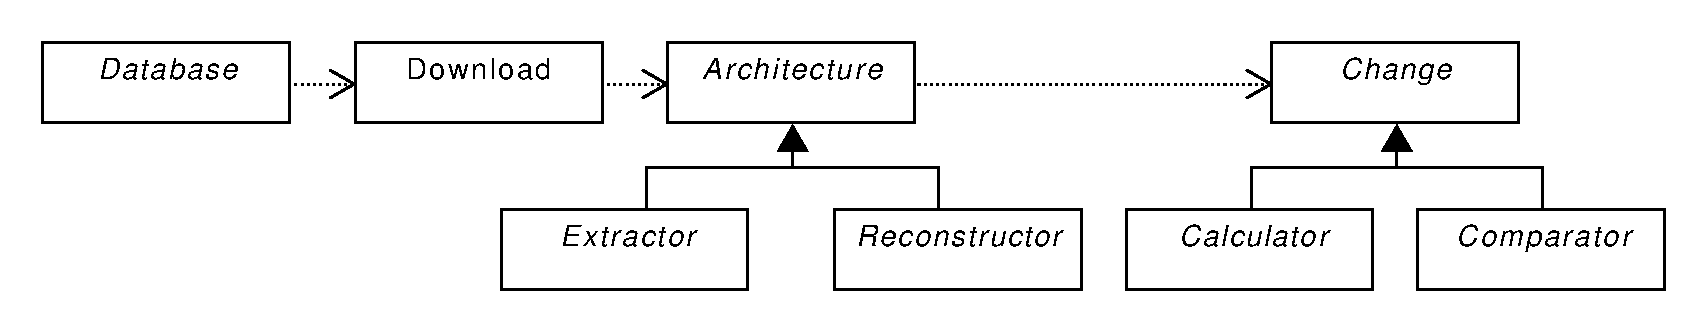
\includegraphics[width=10cm]{assets/architecture.pdf}
\end{block}
}

\only<3>{
\begin{block}{Implemented}
	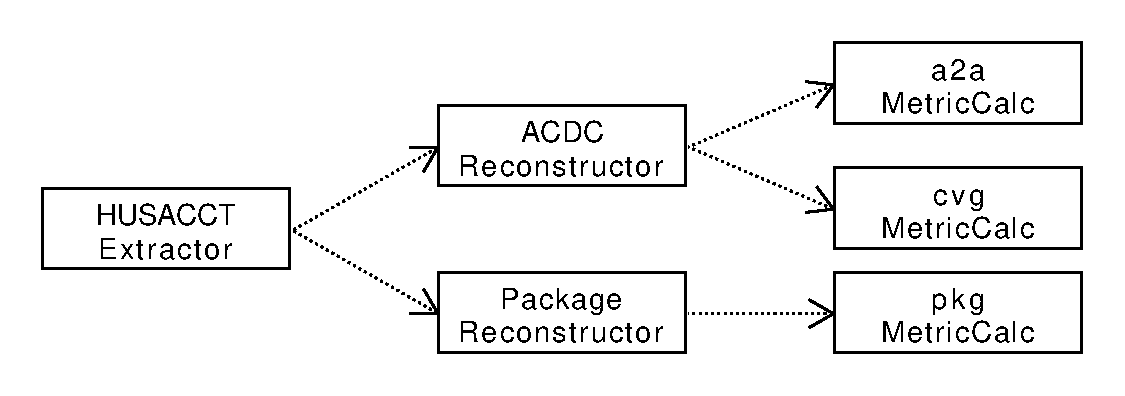
\includegraphics[width=10cm]{assets/implementedArc.pdf}
\end{block}
}

\end{frame}

\subsection{Extracted Results}
\begin{frame}
	\frametitle{Studied Projects}
	
	17380 / 20995 Builds Passed

	\begin{table}
	\caption{Ten Largest Projects under Study}
	\label{tableProjects}
	\centering
	\scalebox{0.9}{
	\begin{tabular}{ | c | c | c | c | c | }
		\hline
		project name & commits & analyzed & range & project type \\
		\hline
		sonarqube & 11590 & 4573 & 1.25y & Code Analyzer \\
		graylog2-server & 8490 & 842 & 4.25y & Log Analyzer \\
		okhttp & 5367 & 1770 & 3.5y & HTTP Client \\
		cloudify & 4984 & 821 & 2.5y & Dev. Framework \\
		structr & 3809 & 1253 & 2.5y & Development App \\
		owlapi & 3238 & 2178 & 3.5y & OWL API \\
		jOOQ & 3196 & 451 & 3y & SQL API \\
		checkstyle & 3029 & 325 & 2y & Code Analyzer \\
		vectorz & 3025 & 46 & 3.5y & Math Library \\
		owner & 2671 & 2099 & 3.5y & Property Files API \\
		\hline
	\end{tabular}
	}
\end{table}


\end{frame}

\begin{frame}
	\frametitle{Metrics}
	\framesubtitle{Correlation}
	
	p values are all 0 

\begin{table}
	\scalebox{0.85}{
	\begin{tabular}{ | c | c | c | c | c | c | c | c | c | }
		\hline
		& \#V & \#E & A. Inst & R. Inst & deg & a2a & cvg src & cvg tar \\
		\hline
		\#V & 1 & 0.93 & 0.58 & 0.59 & 0.69 & 0.23 & 0.45 & 0.49 \\
		\#E & 0.93 & 1 & 0.63 & 0.71 & 0.83 & 0.25 & 0.51 & 0.55 \\
		A. Inst & 0.58 & 0.63 & 1 & 0.81 & 0.43 & 0.2 & 0.44 & 0.46 \\
		R. Inst & 0.59 & 0.71 & 0.81 & 1 & 0.56 & 0.22 & 0.48 & 0.52 \\
		deg & 0.69 & 0.83 & 0.43 & 0.56 & 1 & 0.18 & 0.41 & 0.46 \\
		a2a & 0.23 & 0.25 & 0.2 & 0.22 & 0.18 & 1 & 0.38 & 0.37 \\
		cvg src & 0.45 & 0.51 & 0.44 & 0.48 & 0.41 & 0.38 & 1 & 0.91 \\
		cvg tar & 0.49 & 0.55 & 0.46 & 0.52 & 0.46 & 0.37 & 0.91 & 1 \\
		\hline
	\end{tabular}
	}
\end{table}

\end{frame}

\begin{frame}
	\frametitle{Metrics}
	\framesubtitle{Distribution}
	
	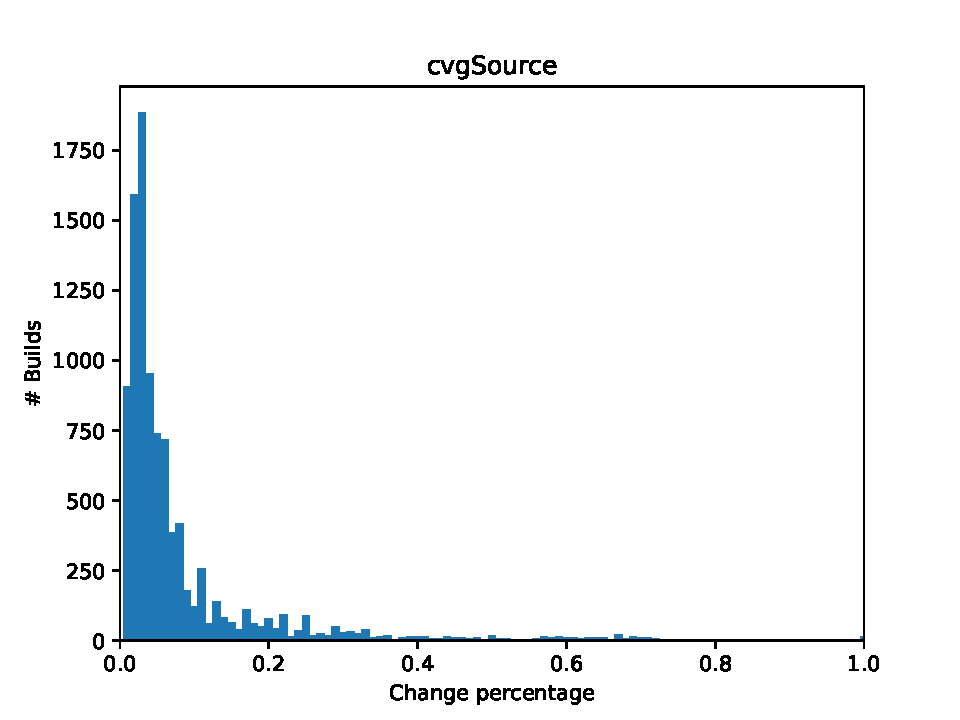
\includegraphics[width=6cm]{assets/cvgSource.pdf}
	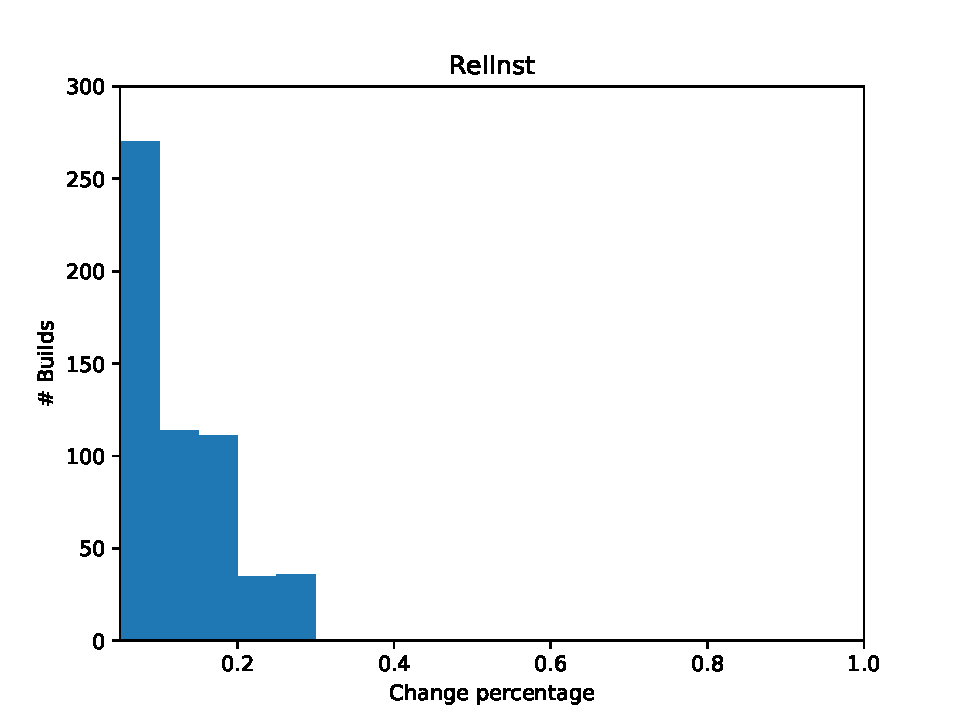
\includegraphics[width=6cm]{assets/RelInst.pdf}
	
\end{frame}

\begin{frame}
	\frametitle{Metrics}
	\framesubtitle{Distribution}
	
	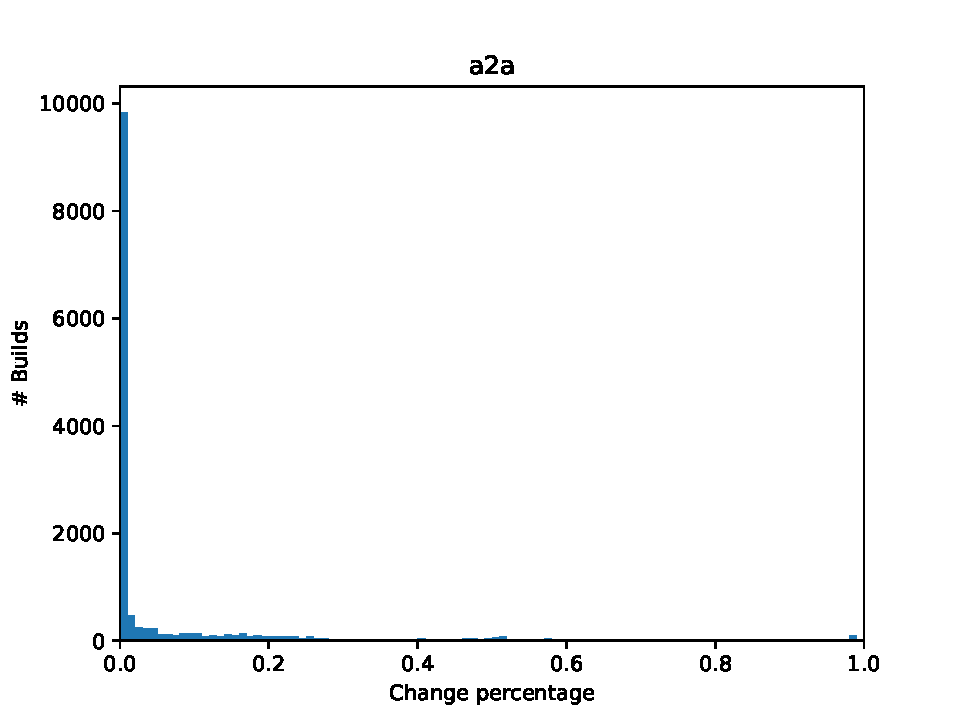
\includegraphics[width=6cm]{assets/a2a.pdf}
	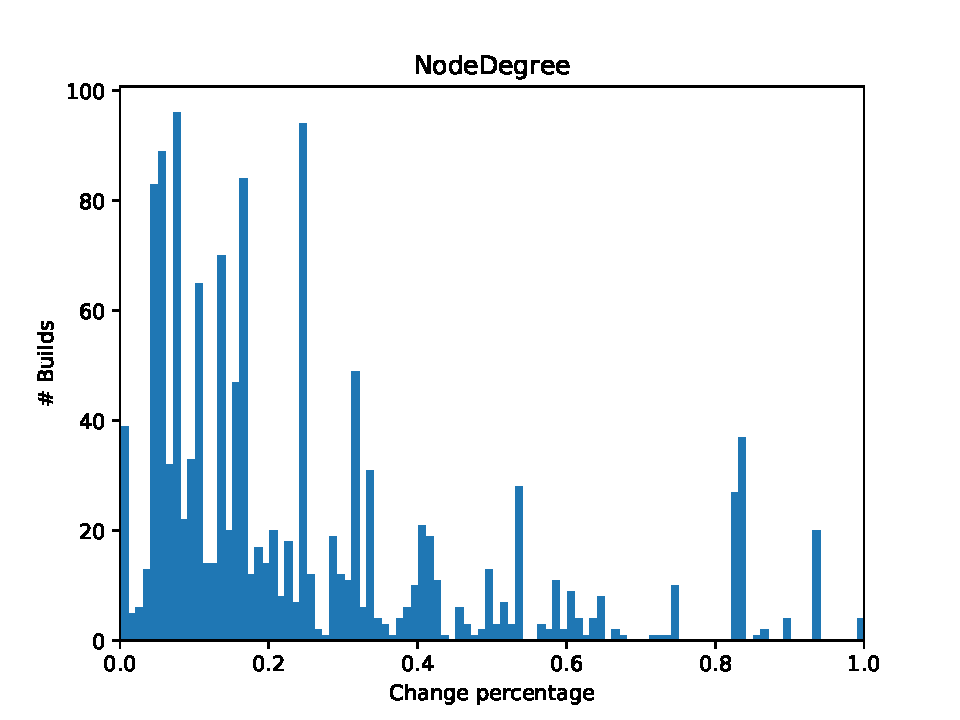
\includegraphics[width=6cm]{assets/NodeDegree.pdf}
	
\end{frame}


\subsection{Correlation}
\begin{frame}
	\frametitle{Correlation}
	
	Calculated Correlations
	\begin{enumerate}
		\item Metric vs Outcome
		\item Metric vs Previous Outcomes
		\item Metric vs Following Outcomes
		\item Change vs Outcome
		\item Change vs Previous Outcomes
		\item Change vs Next Outcomes
	\end{enumerate}
	
	Thresholds for
	\begin{itemize}
		\item Previous / Next: 2, 3, 5, 10
		\item Change: 0.0, 0.01, 0.02, 0.03, 0.04, 0.05, 0.1, 0.2, 0.5
	\end{itemize}
	
\end{frame}

\begin{frame}
	\frametitle{Correlation}
	
	\begin{block}{Results}
		Most Correlations between $0.1- 3\%$
	\end{block}
	\begin{columns}
		\begin{column}{0.5\textwidth}
			Highest Values
			\begin{itemize}
				\item cvg Source / Target
				\item Prev / Next Threshold doesn't matter
			\end{itemize}
		\end{column}
		\begin{column}{0.5\textwidth}
		\begin{center}
			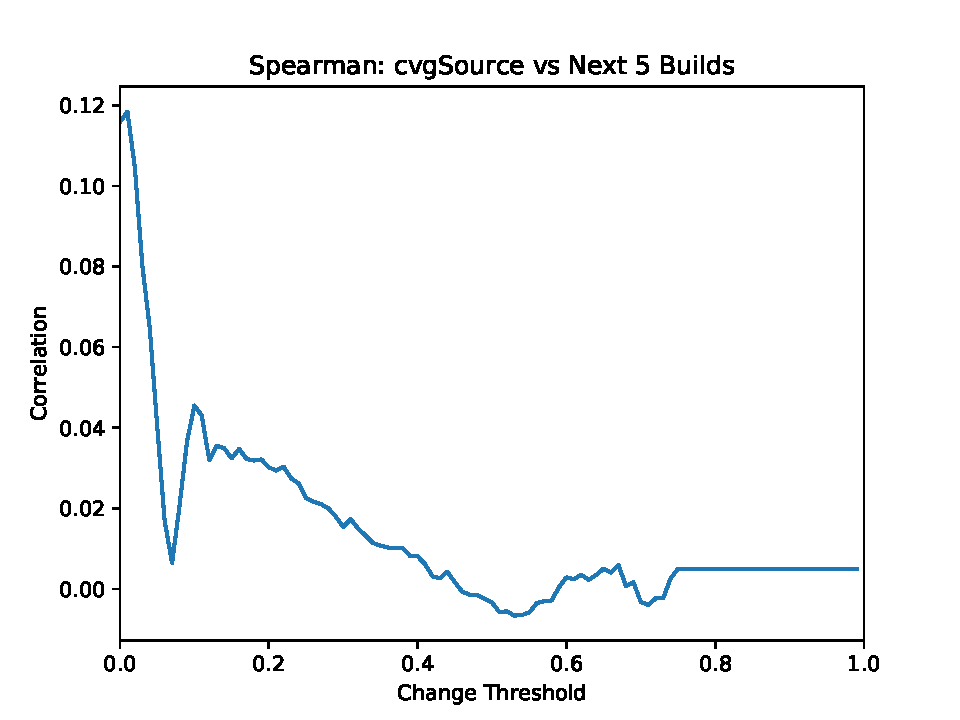
\includegraphics[width=5.5cm]{assets/cvgSourceCorrPlot.pdf}
		\end{center}
		\end{column}
	\end{columns}
	
	
\end{frame}

\section{Interpretation}
\subsection{Implications}
\begin{frame}
\frametitle{Implications}

\begin{itemize}
	\item Projects from different domains and large timescale
	\item Projects from Build 1 and well established
	\item Large number of commits
	\item Low percentage of fails
\end{itemize}
\pause
\begin{itemize}
	\item Metrics follow same pattern
	\item Architecture extraction consistent
\end{itemize}
\pause
\begin{itemize}	
	\item Architecture does not correlate with Build Results
	\item Small impact from changing modules
\end{itemize}

\end{frame}

\subsection{Threats \& Future Work}
\begin{frame}
\frametitle{Threats \& Future Work}

Threats
\begin{itemize}
	\item Only 10 big Java projects
	\item Low amount of build failures
	\item HUSACCT and ARCADE
	\item Wrong metrics
\end{itemize}
\vspace{0.25cm}
\pause

Future Work
\begin{itemize}
	\item More projects
	\item More metrics
	\item More different extractors / reconstructors
\end{itemize}

\end{frame}

\subsection{Summary}
\begin{frame}
\frametitle{Summary}

\begin{itemize}
	\item Large Scale Architecture Reconstruction
	\item easily expendable framework
	\item Almost no correlation between architecture and Build Result
\end{itemize}
\pause
\begin{center}
	
\includegraphics[width=5cm]{assets/professor.jpg}
\end{center}

\end{frame}
 
\end{document}